%! TEX root = **/000-main.tex
% vim: spell spelllang=en:

\section{Extrapolation}%
\label{sec:extrapolation}

It is crucial that we choose an extrapolation method which benifits from the specific properties of our system and solver.
Due to the time constraint on this project we haven't investigated the stability or error bound properties for the extrapolation methods.
While this would be an interesting area to do further research in, we chose methods for which we can safely ignore these properties.
Neuro-VISOR uses the Semi-Implicit Backward Difference 2 method\cite{neuroVISOR}, so linear and quadratic extrapolation are both good options.
To minimize the runtime and memory usage of the extrapolation we've chosen to implement linear extrapolation.

\begin{figure}[H]
    \centering
    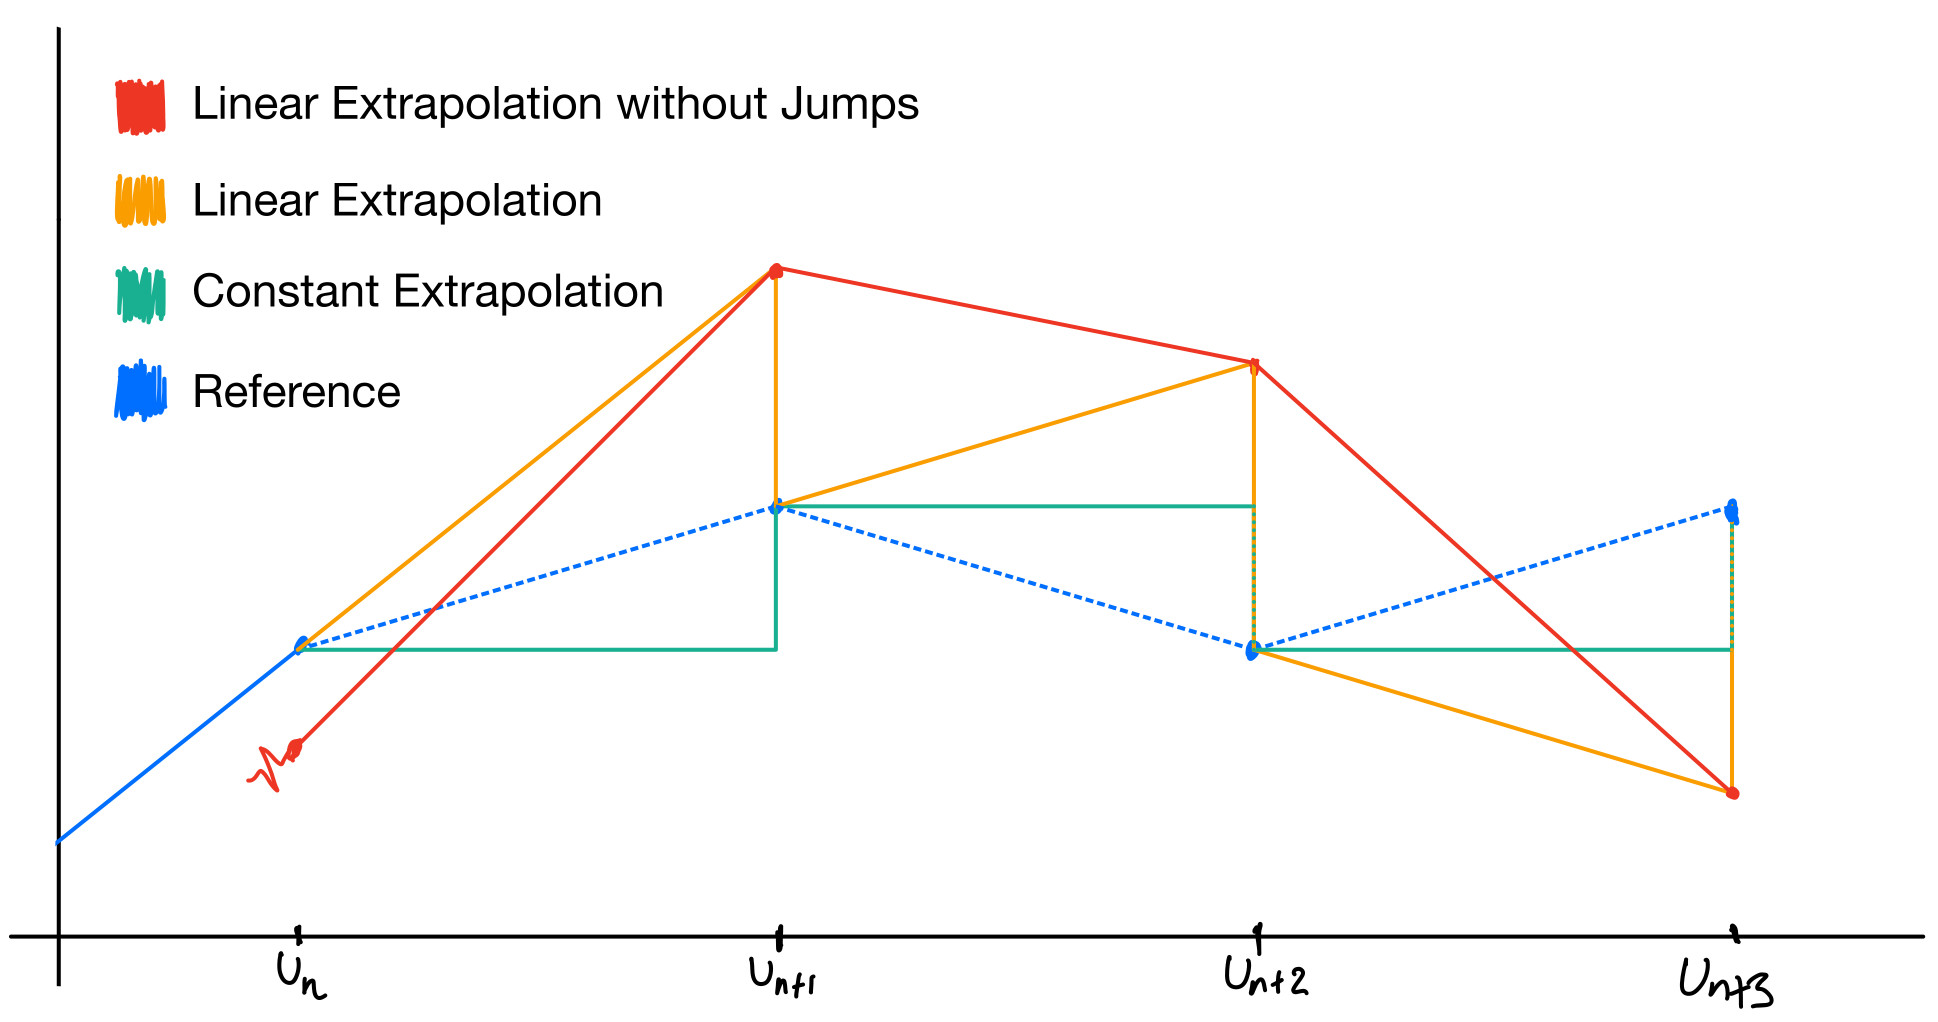
\includegraphics[width=1.0\linewidth]{extrapolationOptions}
    \caption{Linear Extrapolation Methods}%
    \label{fig:extrapMethods}
\end{figure}

\subsection{Optimal Methods}%
\label{sub:optimal_methods}

Linear extrapolation requires a linear function defined in terms of the previous data points.
We can think of linear extrapolation as a family of linear functions $\hat{u}_t : \mathbb{N} \to \mathbb{R}$ parameterized by $t \in [0,1]$ where $\hat{u}_t(n)$ is the point to which the point $u_n$ has moved at time $t$.
The naive definition would be $\hat{u}_t(n) = u_n$ when $t \in [0,1)$ and $\hat{u}_1(n) = u_{n+1}$, which can be seen in \cref{fig:extrapMethods} in green.
Technically Neuro-VISOR implements this when the visualization updates more frequently than the simulation.
Another option is to use $\hat{u}_t(n) = (1-t)u_n + t(2u_n - u_{n-1})$ when $t \in [0,1)$ and $\hat{u}_1(n) = u_{n+1}$, which corresponds to yellow in \cref{fig:extrapMethods}.
A third option is $\hat{u}_t(n) = (1-t)(2u_{n-1} - u_{n-2}) + t(2u_n - u_{n-1})$, which can be seen as red in \cref{fig:extrapMethods}.

As mentioned in the introduction, the goal of this project is to improve the visualization and user experience of the program during unexpected slow downs.
While this is not rigorously defined, we will suppose abrupt jumps decrease the user's experience.
This seems like a reasonable heuristic as abrupt jumps are jarring and make it difficult to follow the simulation.
Constant extrapolation results in a jump whenever $\lim_{t\to1}\hat{u}_t(n) = u_n \not= u_{n+1} = \hat{u}_1(n)$, that is whenever the simulation isn't constant.
``Linear extrapolation with jumps'' results in a jump whenever $\lim_{t\to1}\hat{u}_t(n) = 2u_n - u_{n-1} \not= u_{n+1} = \hat{u}_1(n)$.
In other words, a jump will occur whenever $u_{n+1}$ lies on the line which contains $u_{n-1}$ and $u_n$.
``Linear extrapolation without jumps'' will never result in a jump by definition, as $\hat{u}_1(n) := 2u_n - u_{n-1} =: \hat{u}_0(n+1)$.
While ``linear extrapolation without jumps'' will never jump, accuracy could be an issue when compared to ``linear extrapolation with jumps''.
For example, \cref{fig:l1} shows plots of the L1 norms for the same configuration save one using linear extrapolation with jumps and the other using linear extrapolation without jumps.
The configuration takes values of $\hat{u}_t(n)$ at $0.1$ intervals for $t$ and receives every 10th data point.
The L1 norm graph of the linear extrapolation with jumps has a characteristic sawtooth shape due to it's value being set to the real data point every ten steps.
On the other hand, the L1 graph of the linear extrapolation with jumps will approach the value the other graph approaches before each jump due to it's definition.
Because the error bounds of the linear extrapolation with jumps is smallest when $t=0$, linear extrapolation without jumps will be generally less accurate overall.
These are the three methods that are implemented in our codebase.

\begin{figure}[H]
    \centering
    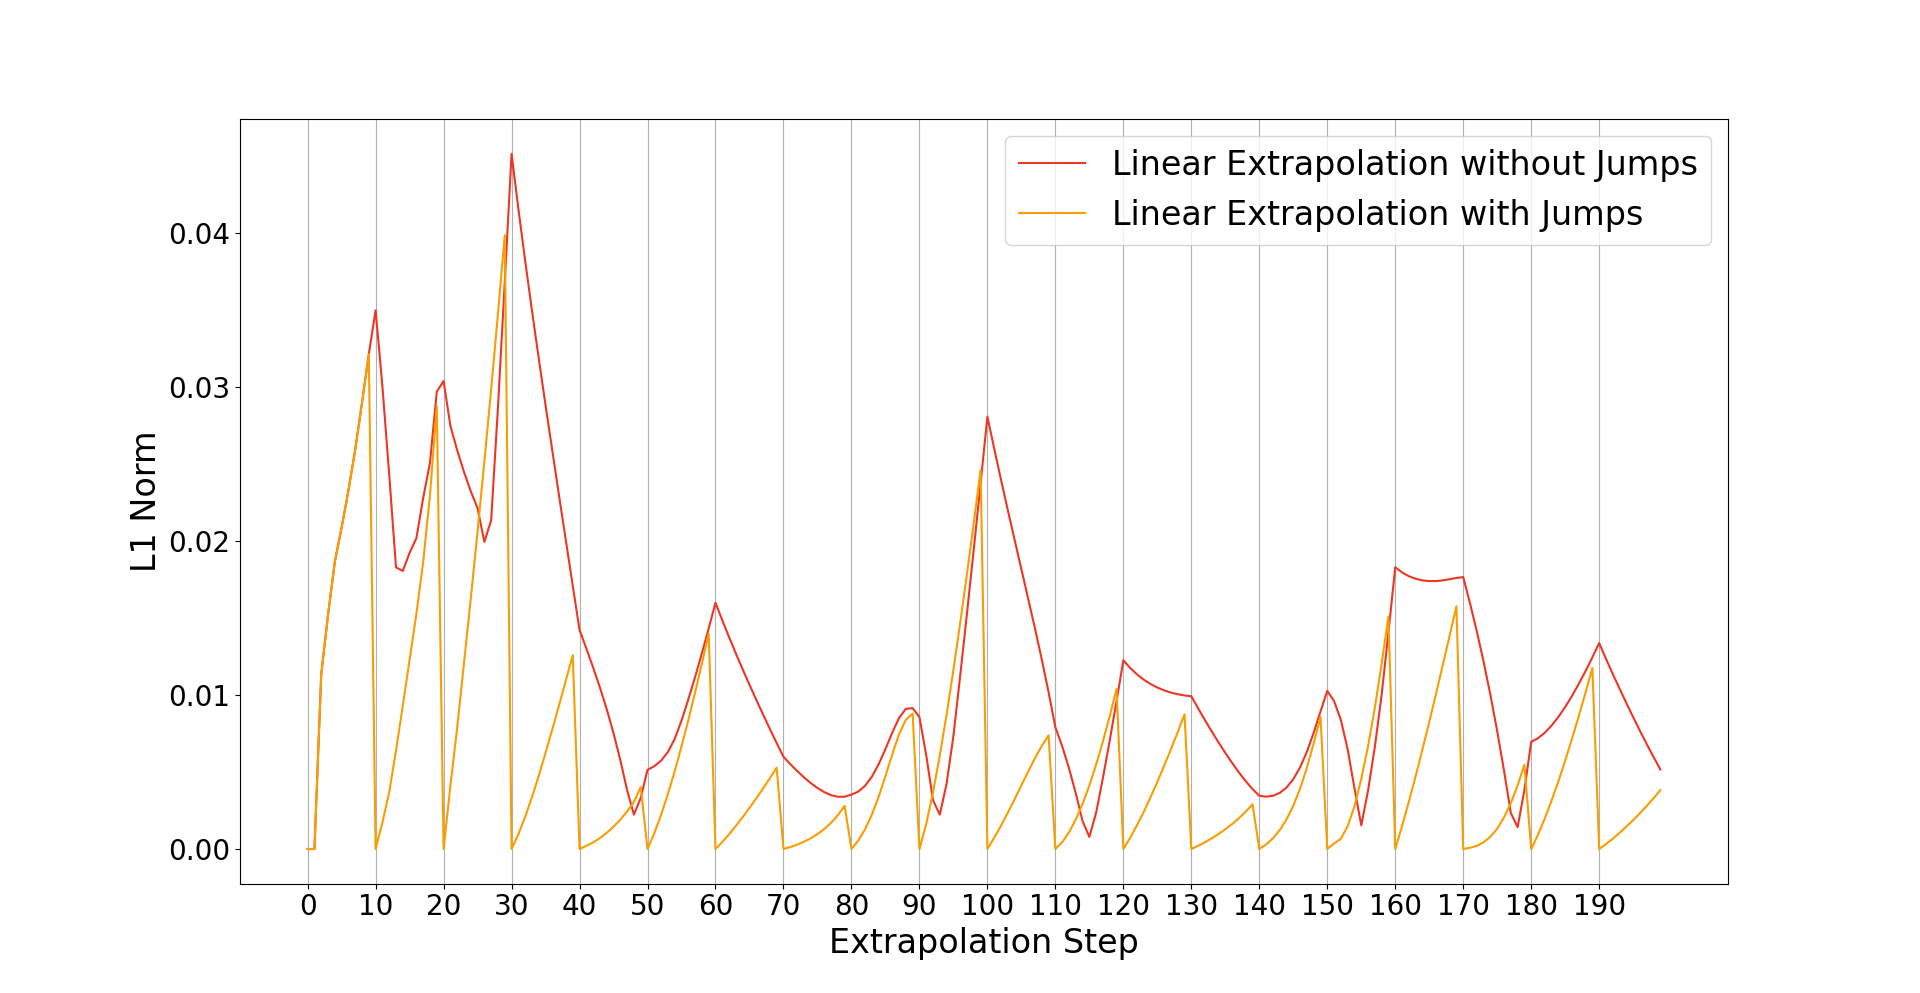
\includegraphics[width=1.0\linewidth]{endpointFull_bothFixedColor}
    \caption{L1 Norms for Linear Extrapolations}%
    \label{fig:l1}
\end{figure}


\subsection{Next Steps}%
\label{sub:next_steps}

The two extrapolation methods that we have focused on are not necessarily the best options.
They both have their pros and cons, however there may be ways of defining linear functions which don't contain jumps but have smaller error bounds.
For example, one could cap the distance between the point used and the previous data point.
Another way could be to define the slope using both the tangent slope and the distance between the starting point and previous data point.
This is an interesting area for future study, especially showing rigorous results in this area and exploring non-linear options.
